% !TEX root = ../SCXMLREF.tex

\section{Verification of Intrusion Detection System}
\label{sec:example}

One of our main goals is to express properties in \SCXML intermediate refinements and prove them via translation to \EventB.
In this section we illustrate how this can be done in the \IDS example.

Properties about the synchronisation of parallel state-machines (such as |Go = TRUE => Idle = TRUE|)
% and |ASIC=Wait50ms => SPI=IDLE|
can be difficult to verify for all scenarios via simulation in \SCXML. 
Proof of such properties is a major benefit of translating into Event-B.  
Furthermore,  in order to benefit from the abstraction provided by Event-B, we would like to prove such things at abstract levels before the complication of further details are introduced. 
Typically these further details concern the raising of internal triggers that contribute to the synchronisation we wish to verify. 
Therefore additional constraints, that are an abstraction of the missing details, are needed about triggers in order to perform the proof.
% \begin{figure}[!tbp]
\begin{figure}[!h]
	\vspace{-.4cm}
	\centering
	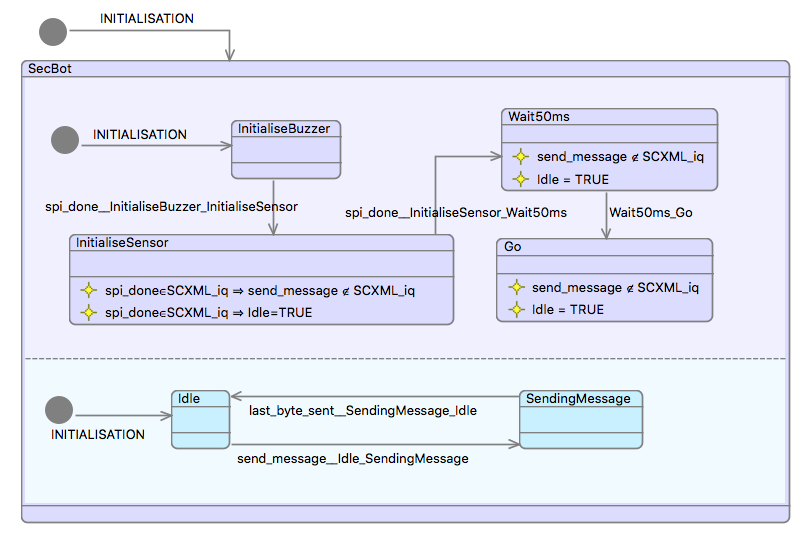
\includegraphics[width=0.8\textwidth]{figures/iumlb_verif}
	\caption{State invariants to be verified at refinement level 1.}
	\label{fig:iumlb-verif}
	\vspace{-.4cm}
\end{figure}

\begin{sloppypar}
Fig.~\ref{fig:iumlb-verif} is the generated \iUMLB showing state invariants (textual properties with a star icon inside states) to be verified. Note that the invariants are added to the \SCXML model but are easier to visualise in the \iUMLB with the current tooling.
The main aim is to show the property |Idle=TRUE| holds in state |Go|. 
This is true because after sending the message while in |InitialiseSensor|, no other messages are triggered by the |ASIC|, so the |SPI| subsystem stays in the |Idle| state indefinitely. 
To enable the provers to discharge the proof obligation we work back along the |ASIC|'s sequence of states. 
That is, |Idle = TRUE| is maintained in state |Go| if it holds in state |Wait50ms| and no |send_message| triggers are raised by the entry transition |Wait50ms_Go| nor once the |ASIC| subsystem is in state |Go|. 
To ensure this we add a guard |send_message /: SCXML_raisedTriggers| to |Wait50ms_Go| to prevent any future refinement from raising the trigger |send_message|.
(Currently, this is added verbatim but we envision a `doesn't raise' notation to avoid the user having to reference the translation artefact, |SCXML_raisedTriggers|).
We also need to prevent any future transitions from raising this trigger in the state |Go|.
To automate this for all abstract `future' events, they could be automatically generated and added to satisfy all user invariants concerning the raising of internal triggers regardless of whether they are violated in future levels. 
For example, the guard  |Go = TRUE => send_message /: SCXML_raisedTriggers| needs to be automatically added to the three `basis' events,
 |SCXML_futureUntriggeredTransitionSet|, |SCXML_futureInternalTransitionSet| and |SCXML_futureExternalTransitionSet| to prove they do not break the property being verified. 
If it is not obeyed by future transitions, guard strengthening proof obligations will fail, making it obvious where the problems lie.
As indicated above, we now need to prove by similar means that |Idle=TRUE| holds in state |Wait50ms|. 
In this case, however, we can only say that |Idle=TRUE| in state |InitialiseSensor| after the \SPI-system finishes sending the message and raises the trigger, |spi_done|. 
Hence the state invariant for |InitialiseSensor| becomes |spi_done∈SCXML_iq => Idle=TRUE|. 
In order to prove this we again need a corresponding state invariant about |send_message| and need to make sure that the |SPI| system will never raise |send_message|.
We also ensure it does not raise |spi_done| until it is finished. 
With these invariants and additional guards the Rodin automatic provers are able to prove all proof obligations and hence verify that the |SPI| system remains in |Idle| after servicing the `Initialise Sensor' message.
\end{sloppypar}

In order to prove properties at an abstract level we constrain the behaviour to be added in later refinements. 
For example, we needed to add a guard to specify that a transition does not raise a particular trigger in any future refinement. 
The abstract constraints should not appear in later refinements when the details have been finalised. To do this we could introduce ranges into our refinement attributes.

%%% Local Variables:
%%% mode: latex
%%% TeX-master: "../SCXMLREF"
%%% End: